\section{Baseline}
\label{sec:Baseline}
In this section, we analyze the results obtained from applying our methodologies on synthetic data and establish their efficacy.

\subsection{Ground truth: Task $1_a$}
\label{sec:Ground truth: Task $1_a$}
\graphicspath{{pictures/task1a/}}
For task1\textsubscript{a}, we use $\Omega_1$ as our synthetic data and calculate the 10 most negatively correlated and 10 most positively correlated features with $Death$.

\begin{figure}[H]
  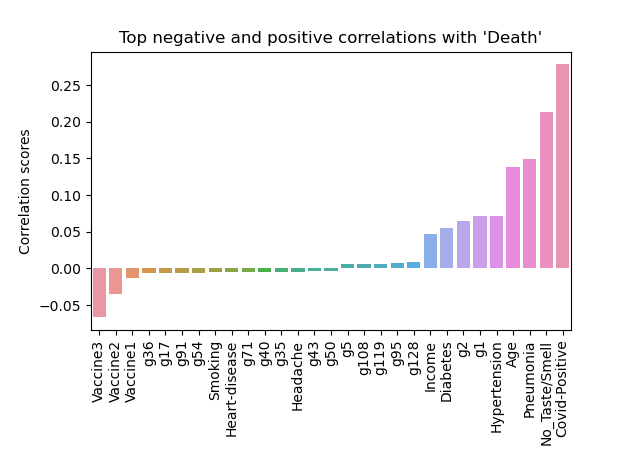
\includegraphics[width=\linewidth]{1a1.png}
  \caption{Correlations between Death and other features for the set $\Omega_1$.}
    \label{fig:1a1}
\end{figure}
In Figure \ref{fig:1a1} we look at the correlation between $Death$ and some of our features. As expected, vaccines are the most negatively correlated with $Death$, especially $Vaccine3$, which seems to be the most efficient. On the other hand, $CovidPositive$ appears most predictive of death, followed by some symptoms. 

\begin{figure}[H]
  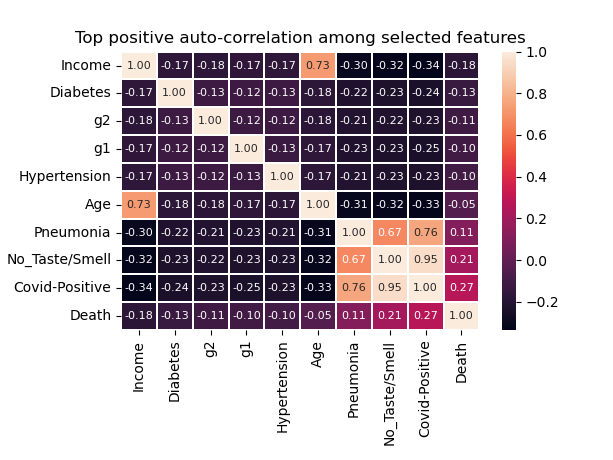
\includegraphics[width=\linewidth]{1a2.png}
  \caption{Auto-correlations among features for the set $\Omega_1$.}
  \label{fig:1a2}
\end{figure}

In Figure \ref{fig:1a2}, we observe the auto-correlations between features. We notice a high correlation between $CovidPositive$ and some symptoms, such as $No\_Taste/Smell$ and $Pneumonia$. In addition, there is a high auto-correlation between $Income$ and $Age$. For this reason, we consider only the $CovidPositive$ population and remove the $Income$ variable from this data to obtain all independent explanatory variables, which is a necessary assumption for our chosen $Logistic$ $Regression$ model. 
%Reference this section in the results, because this happens in the real data

\begin{figure}[H]
  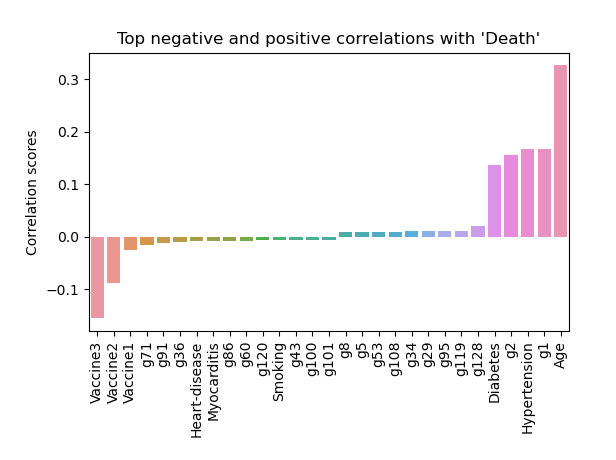
\includegraphics[width=\linewidth]{1a3.png}
  \caption{Correlations between $Death$ and selected features for the set $\Omega_1$.}
  \label{fig:1a3}
\end{figure}

At this point, we observe the new \textbf{Figure \ref{fig:1a3}} containing a distinct correlation-rank. Indeed, there is a significant difference from \textbf{Figure \ref{fig:1a1}}, because previously the feature $CovidPositive$ brought some auto-correlated symptoms to the top-correlated features with $Death$. This is to say that, since $CovidPositive$ is highly correlated to $Death$ and some symptoms are auto-correlated to $CovidPositive$, then these symptoms seemed to also be correlated with $Death$. However, this logic contradicts the underlying process to generate the synthetic data and is not desirable. When we analyze the data within the $CovidPositive$ population, we can then notice that these specific symptoms do not explain $Death$, but only $CovidPositive$. Under this analysis, the auto-correlated symptoms features disappear from the top-ranked and are replaced by other variables that actually explain $Death$ according to our design of the synthetic data.

Our results here establish that methodology\textsubscript{1} can reliably identify features which affect patient outcomes either positively or negatively. The method reliably and correctly identifies the known positive relationship between the $Age$, $Gene_1$, $Hypertension$, $Gene_2$, $Diabetes$ features with $Death$ as we defined in the synthetic data generation.

%Methodology 2 section for this part
Following methodology\textsubscript{1}, we then apply methodology\textsubscript{2} on $\Omega_1$. 

\begin{figure}[H]
  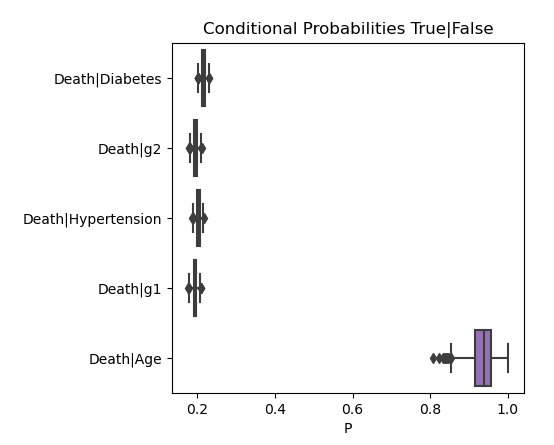
\includegraphics[width=\linewidth]{1a7.png}
  \caption{Conditional Probability of Death in $\Omega_1$ without comorbidities.}
  \label{fig:1a7}
\end{figure}

\begin{figure}[H]
  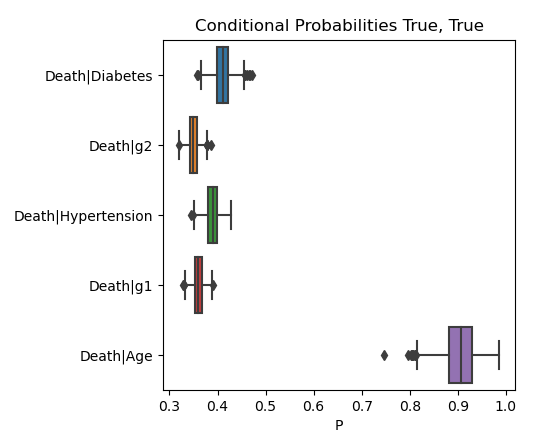
\includegraphics[width=\linewidth]{1a8.png}
  \caption{Conditional Probability of Death in $\Omega_1$ with comorbidities.}
  \label{fig:1a8}
\end{figure}

In \textbf{Figures \ref{fig:1a7}} and \textbf{\ref{fig:1a8}} we observe the conditional probability when comorbidities are not present and present, respectively. The conditional probability of death is observed to be higher when $Diabetes$ and $Hypertension$ are present, as well as with $Gene_1$ and $Gene_2$. In the latter case, the effect appears less pronounced, however in our synthetic data it is the combined presence of both genes that increases the probability of death, so individually their impact on the chance of death is less noticeable in this methodology. Nonetheless, the features which cause death in our synthetic data are correctly identified and the increased effect on death is clearly shown over the 1000 probability estimates.

%Write Methodology 3 section under here for this section
Finally we apply methodology\textsubscript{3} to $\Omega_1$. 

\begin{figure}[H]
  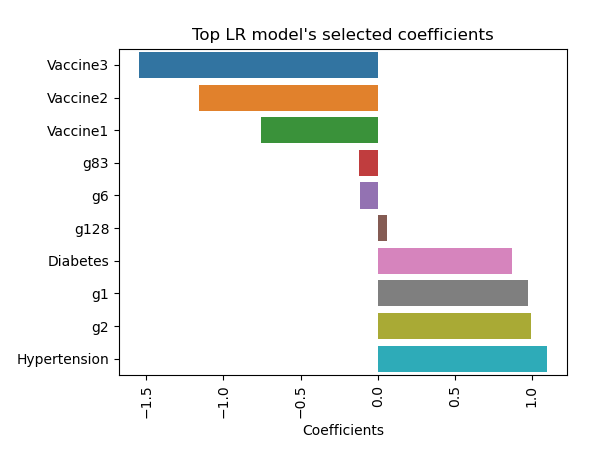
\includegraphics[width=\linewidth]{1a9.png}
  \caption{Coefficient Values of Logistic Regression on $\Omega_1$, after randomized grid-search 500-fold CV.}
  \label{fig:1a9}
\end{figure}

\begin{figure}[H]
  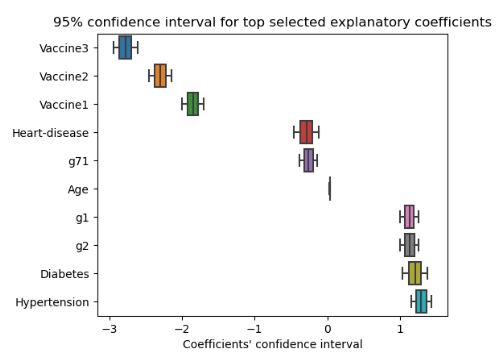
\includegraphics[width=\linewidth]{1a10.png}
  \caption{95\% Confidence Interval for Logistic Regression Coefficient Values.}
  \label{fig:1a10}
\end{figure}

As described in Section \ref{sec:methodologies}, we train a $Logistic$ $regression$ classifier to predict $Death$. The best performing model scored an accuracy of $0.82$, and we then observed the coefficient values of the model. In \textbf{Figure \ref{fig:1a9}}, we show the 5 largest positive and 5 largest negative coefficient values for the classifier. The vaccines have by far the largest negative coefficient value in predicting $Death$, as expected. On the other side, $Hypertension$, $Gene_2$, $Gene_1$, and $Diabetes$ are the most useful features for the model to predict $Death$. We can then conclude that as with the first two methodologies, methodology\textsubscript{3} accurately identifies the features which predict death and our overall framework for analyzing the real data is robust.

%End of this section
\subsection{Ground truth: Task $1_b, 1_c$}
\graphicspath{{pictures/task1b/}}
In this subsection we use another synthetic dataset $\Omega_2$, in which we imposed a correlation between each vaccine and a specific side effect.

\begin{figure}[H]
  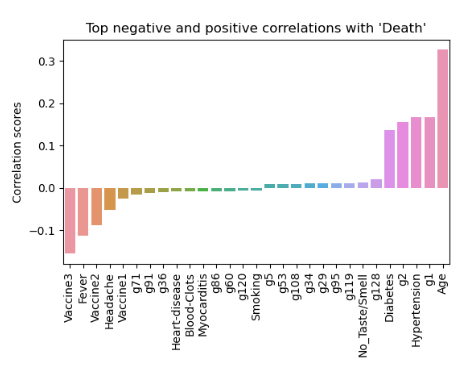
\includegraphics[width=\linewidth]{1b1.png}
  \caption{Correlations between Death and selected features for the set $\Omega_2$.}
    \label{fig:1b1}
\end{figure}

Similarly to \textbf{Figure \ref{fig:1a1}}, in \textbf{Figure \ref{fig:1b1}} we observe the positive and negative correlations between features and death. These two figures are very similar, with the exception that side-effects from the vaccines now appear among negatively correlated features. These results are consistent with the generation of $\Omega_2$ as described in Section \ref{sec:synthetic_data}.

%Write Methodology 2 for this task below here (shorter than before since it's already described in the previous subsection)

\begin{figure}[H]
  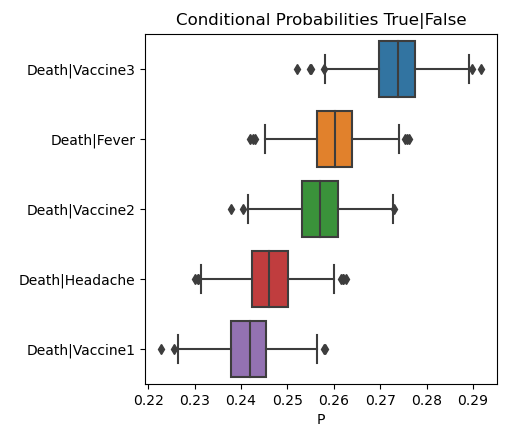
\includegraphics[width=\linewidth]{1b5.png}
  \caption{Conditional Probability of Death in $\Omega_2$ without comorbidities.}
  \label{fig:1b5}
\end{figure}

\begin{figure}[H]
  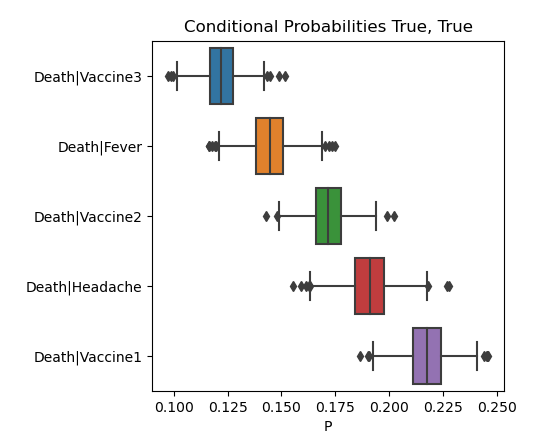
\includegraphics[width=\linewidth]{1b6.png}
  \caption{Conditional Probability of Death in $\Omega_2$ with comorbidities.}
  \label{fig:1b6}
\end{figure}

\textbf{Figures \ref{fig:1b5}} and \textbf{\ref{fig:1b6}} again show the effect of the vaccines in reducing the likelihood of death, as defined for $\Omega_2$. We then also investigate the conditional probability of symptoms given vaccines.

\graphicspath{{pictures/task1c/}}

\begin{figure}[H]
  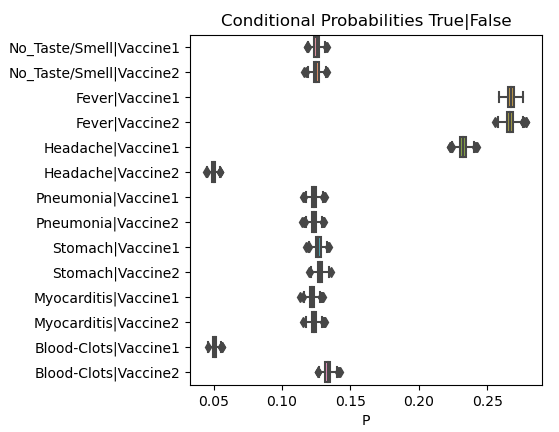
\includegraphics[width=\linewidth]{1c3.png}
  \caption{Conditional Probability of Symptoms in $\Omega_2$ without comorbidities.}
  \label{fig:1c3}
\end{figure}

\begin{figure}[H]
  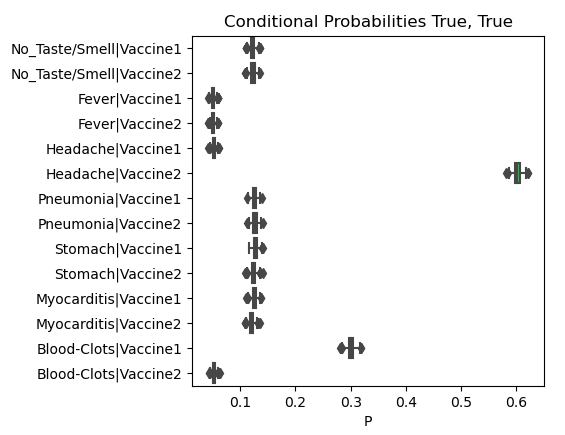
\includegraphics[width=\linewidth]{1c4.png}
  \caption{Conditional Probability of Symptoms in $\Omega_2$ with comorbidities.}
  \label{fig:1c4}
\end{figure}

These plots show the side-effect we defined for two of the vaccines (omitting $Vaccine3$ for purposes of space) in $\Omega_2$. The chance of having a $Headache$ is accurately shown to be affected by $Vaccine2$, and likewise the relationship between $Blood\_Clot$ and $Vaccine1$.

%Write Methodology 3 for this task below here (shorter than before since it's already described in the previous subsection)

Lastly, we analyze $\Omega_2$ with our third methodology. As in Task $1a$\textsubscript{\ref{sec:Ground truth: Task $1_a$}}, the model is able to learn the correct features to predict $Death$, which are the same as before because we are training the model to predict the same outcome. We can then conclude that our methods analyze the $\Omega_2$ synthetic data appropriately.

\subsection{Ground truth: Task$_2$}
\graphicspath{{pictures/task2/}}
For task$_2$, we use $\Omega_3$ as our synthetic data. In this subsection we are interested in the effect of treatments on alleviating symptoms and preventing deaths.

%Methodology 1

\begin{figure}[H]
  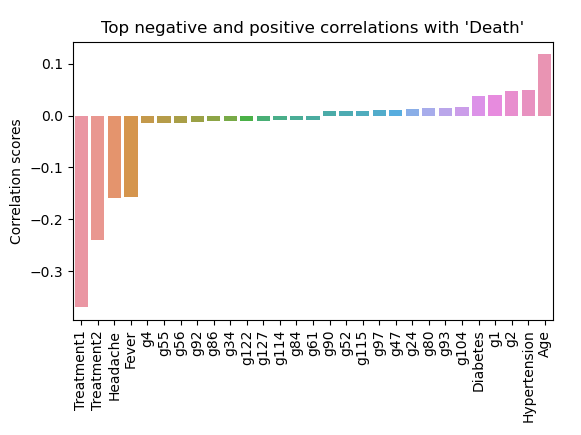
\includegraphics[width=\linewidth]{2_1.png}
  \caption{Correlations between $Death$ and other features for $\Omega_3$.}
    \label{fig:2_1}
\end{figure}

In \textbf{Figure \ref{fig:2_1}} we examine the top negative and positive correlations with $Death$. As expected, among the top negative features we find the two treatments while in the positive features we observe $Age$, $Hypertension$, $Gene_1$, $Gene_2$ and $Diabetes$. We defined the data such that both treatments are effective, with $Treatment 1$ being more effective (thus both are highly negatively correlated to death). Additionally, $Treatment 1$ is associated with a side effect of $Headache$ and $Treatment 2$ is associated with a side effect of $Fever$ and these features are thereby negatively correlated with $Death$ due to their auto-correlation with the treatments. 

%Methodology 2
\begin{figure}[H]
  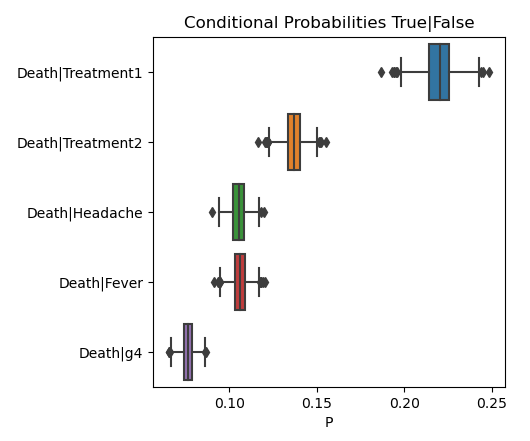
\includegraphics[width=\linewidth]{2_5_top.png}
  \caption{Conditional Probability of Death in $\Omega_3$ without comorbidities.}
    \label{fig:2_5}
\end{figure}

\begin{figure}[H]
  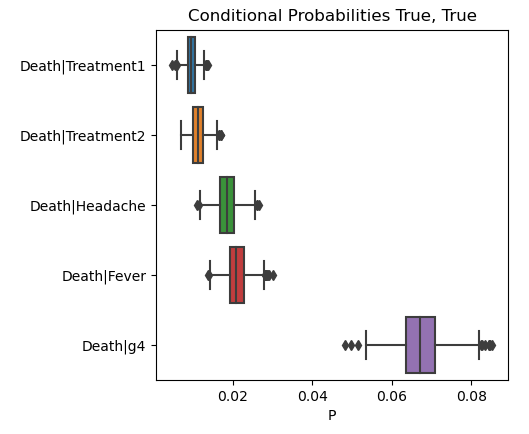
\includegraphics[width=\linewidth]{2_6_top.png}
  \caption{Conditional Probability of Death in $\Omega_3$ with comorbidities.}
    \label{fig:2_6}
\end{figure}

Methodology 2 as applied to $\Omega_3$ shows the influence of treatment on the chance of death. When treatments are not applied, the chance of death is above $14\%$ as in \textbf{Figure \ref{fig:2_5}}, both treatments are given, the probability of death is reduced to $0.01$ as in \textbf{Figure \ref{fig:2_6}}. Each treatment also individually reduces the chance of death. \textbf{Figure \ref{fig:2_6_after}} shows the probability of symptoms after treatment has been applied. Treatments predict each other's side effects because it is possible for a patient to be treated with both.

\begin{figure}[H]
  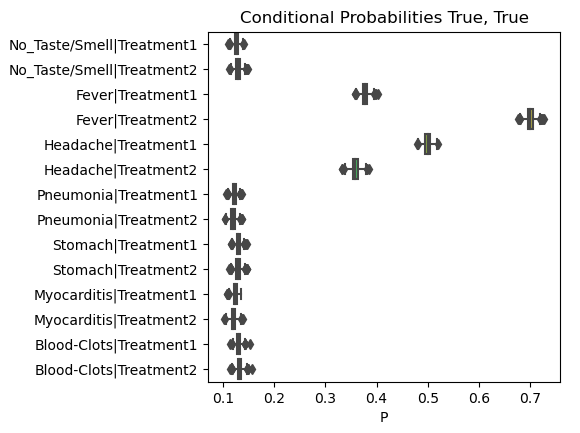
\includegraphics[width=\linewidth]{2_6_after.png}
  \caption{Conditional Probability of Symptoms Given Treatments for $\Omega_3$.}
    \label{fig:2_6_after}
\end{figure}

%Methodology 3

Our final test on synthetic data is applying methodology\textsubscript{3} to $\Omega_3$. The methodology here returns the coefficient values for a $Logistic$ $regression$ model predicting death given treatment.

\begin{figure}[H]
  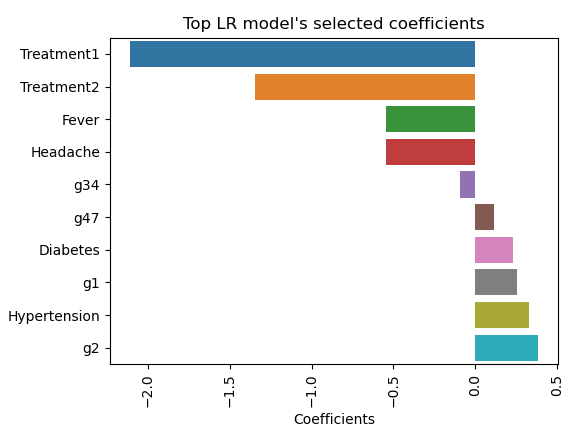
\includegraphics[width=\linewidth]{2_11.png}
  \caption{Coefficient Values of Logistic Regression on $\Omega_3$, after randomized grid-search 500-fold CV.}
    \label{fig:2_11}
\end{figure}

\begin{figure}[H]
  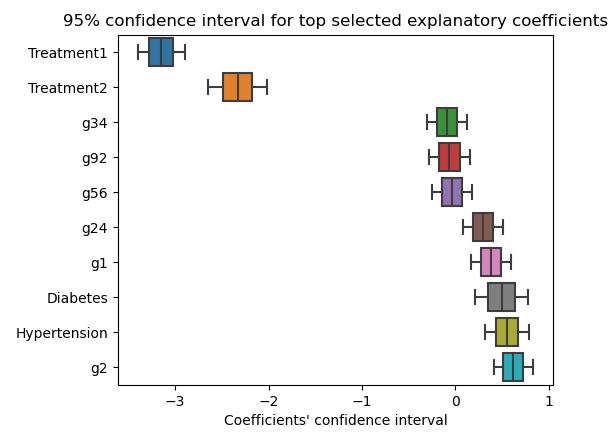
\includegraphics[width=\linewidth]{2_12.png}
  \caption{95\% Confidence Interval for Logistic Regression Coefficient Values.}
    \label{fig:2_12}
\end{figure}

In \tetbf{Figure \ref{fig:2_11}} we show the top positive and negative coefficient values for this model. The best model accuracy for this data was $0.86$. These coefficients accurately show that treatments are highly predictive of survival in $\Omega_3$. \textbf{Figure \ref{fig:2_12}} shows the confidence interval for the coefficient values, showing that the model training procedure results in a useful range of values that allow the correct conclusion to be drawn that treatments are effective.

Therefore, given all of the experiments performed on the three synthetic datasets, we are able to determine that each of our methodologies are capable of inferring the correct conclusions to explaining the synthetic data and match how we created this data.
